% ==========================================
% BAB IV PERANCANGAN
% ==========================================
\cleardoublepage
\chapter{PERANCANGAN}
\label{chap:perancangan}

\section{Deskripsi Umum Sistem}
Sistem manajemen akses karyawan yang dikembangkan merupakan solusi \textit{middleware} yang menjembatani perangkat keras terminal biometrik dengan sistem informasi terpusat. Desain konsep sistem baru ini berfokus pada penghapusan sekat data (\textit{data silo}) dan peningkatan visibilitas operasional melalui antarmuka berbasis web yang responsif. Sebagai solusi \textit{middleware}, sistem ini dirancang bersifat non-invasif, di mana kehadirannya tidak menggantikan atau mengganggu operasional perangkat lunak vendor (\textit{existing}) yang sudah terpasang, melainkan berjalan secara paralel sebagai jalur agregasi data otomatis.

\subsection{Model Konseptual Perbandingan}
Perbedaan fundamental antara sistem kontrol akses saat ini (\textit{existing}) dengan sistem yang diusulkan (\textit{proposed}) terletak pada aliran data dan metode aksesnya. 

\begin{enumerate}
    \item Sistem Saat Ini (Manual/Isolated): Data log dan profil karyawan tersimpan secara lokal pada terminal dan PC Resepsionis. Pengelola harus melakukan ekspor data manual untuk setiap kebutuhan pelaporan, dan pemantauan hanya dapat dilakukan dari satu titik fisik menggunakan perangkat lunak \textit{proprietary}.
    \item Sistem yang Diusulkan (Automated/Web-based): Server \textit{backend} (NestJS) bertindak sebagai pusat kendali otomatis yang secara periodik menarik log pergerakan dan menyinkronkan data identitas biometrik melalui protokol ISAPI. Data disimpan dalam basis data PostgreSQL terpusat, sehingga informasi dapat diakses secara \textit{real-time} melalui peramban web dari seluruh jaringan gedung.
\end{enumerate}

Untuk memberikan gambaran yang lebih jelas mengenai keunggulan sistem yang diusulkan, Tabel \ref{tab:perbandingan_sistem} merangkum perbandingan fitur antara kedua sistem tersebut.

\begin{table}[H]
    \centering
    \caption{Perbandingan Fitur Sistem Eksisting vs Sistem yang Diusulkan}
    \label{tab:perbandingan_sistem}
    \begin{tabular}{|l|p{6cm}|p{6cm}|}
        \hline
        \textbf{Aspek} & \textbf{Sistem Eksisting (iVMS-4200)} & \textbf{Sistem yang Diusulkan} \\
        \hline
        Aksesibilitas & Terbatas hanya pada satu PC lokal di area lobi. & Fleksibel via peramban web di seluruh jaringan gedung. \\
        \hline
        Sinkronisasi Data & Bergantung pada proses manual atau tarikan otomatis aplikasi vendor. & Otomatis dan berkesinambungan menggunakan algoritma \textit{Mark \& Sweep}. \\
        \hline
        Penyimpanan Log & Terisolasi dalam basis data lokal PC Resepsionis. & Terpusat dalam basis data PostgreSQL untuk agregasi BGC. \\
        \hline
        Investigasi Anomali & Memerlukan pengecekan manual pada layar terminal atau PC lobi. & Otomatis menyajikan foto \textit{snapshot} wajah pada \textit{dashboard} admin. \\
        \hline
        Keamanan Siber & Bergantung sepenuhnya pada keamanan PC lokal. & Dilindungi oleh lapisan \textit{Reverse Proxy} dan otentikasi terpusat. \\
        \hline
    \end{tabular}
\end{table}

\section{Arsitektur Sistem}
Perancangan arsitektur sistem pada penelitian ini dibagi menjadi dua aspek utama: arsitektur perangkat lunak yang mengatur pemisahan logika program, dan arsitektur jaringan yang mendefinisikan topologi fisik serta lapisan keamanan siber.

\subsection{Arsitektur Perangkat Lunak (\textit{Software Architecture})}
Sistem ini dirancang menggunakan pendekatan Arsitektur Tiga Lapis (\textit{Three-Tier Architecture}) yang dimodifikasi. Pendekatan ini memisahkan tanggung jawab sistem ke dalam tiga lapisan independen untuk memudahkan skalabilitas dan pemeliharaan:

\begin{enumerate}
    \item Lapisan Presentasi (\textit{Client Tier}): Dibangun menggunakan kerangka kerja \textit{Next.js}. Lapisan ini bertanggung jawab untuk merender antarmuka pengguna (\textit{dashboard}) di sisi peramban. Penggunaan pustaka \textit{Socket.IO} pada lapisan ini dipilih karena kemampuannya dalam menangani pemutusan koneksi otomatis (\textit{auto-reconnect}) dan mekanisme \textit{heartbeat} di sisi klien, guna menjamin kestabilan aliran data pergerakan secara \textit{real-time} tanpa membebani server dengan permintaan \textit{polling} HTTP secara terus-menerus.
    \item Lapisan Aplikasi (\textit{Middleware/Logic Tier}): Dibangun menggunakan \textit{NestJS} (Node.js). Lapisan ini merupakan inti komputasi sistem yang bertindak sebagai jembatan (\textit{middleware}). \textit{NestJS} mengelola penjadwalan asinkron (\textit{Cron Jobs}) untuk menarik data log dari perangkat keras via protokol ISAPI, memproses logika anomali (deteksi akses tertolak), dan menyediakan \textit{RESTful API} bagi lapisan presentasi. Sebagai catatan batasan perancangan, sinkronisasi data dari \textit{middleware} ke terminal gerbang saat ini dibatasi pada data tekstual (ID Karyawan, Nama, dan Jenis Kelamin). Pengunggahan data visual wajah secara dua arah ditangguhkan karena adanya isu kompatibilitas pembacaan \textit{multipart/form-data boundary} pada \textit{firmware} Hikvision versi V4.38, sehingga pendaftaran wajah karyawan untuk sementara tetap memanfaatkan pemindai fisik pada terminal.
    \item Lapisan Data (\textit{Data Tier}): Menggunakan \textit{PostgreSQL} sebagai basis data relasional utama untuk menyimpan profil karyawan dan agregasi riwayat akses secara permanen. Lapisan data ini di-\textit{hosting} sepenuhnya pada lingkungan server lokal yang sama dengan lapisan aplikasi untuk menjamin privasi data biometrik dan mencegah kebocoran informasi ke jaringan publik. Lapisan ini juga mencakup mekanisme \textit{file storage} lokal khusus untuk menyimpan bukti tangkapan layar (\textit{snapshot}) pada kejadian akses yang ditolak (anomali).
\end{enumerate}

\subsection{Arsitektur Jaringan dan Keamanan Siber (\textit{Network \& Security Architecture})}
Untuk memenuhi standar keamanan siber Bangunan Gedung Cerdas (BGC), topologi jaringan dirancang agar sistem terisolasi dan terlindungi dari akses publik yang tidak sah. Gambar 4.2 mengilustrasikan topologi jaringan sistem.

\begin{figure}[H]
    \centering
    % \includegraphics[width=0.8\textwidth]{images/arsitektur_jaringan.png}
    \vspace{4cm} % Placeholder tinggi gambar
    \caption{Desain Arsitektur Jaringan dan Lapisan Keamanan}
    \label{fig:arsitektur_jaringan}
\end{figure}

Implementasi keamanan siber pada arsitektur jaringan ini meliputi:
\begin{enumerate}
    \item \textit{Reverse Proxy} (NGINX): Ditempatkan sebagai titik masuk tunggal (\textit{single point of entry}) bagi seluruh permintaan HTTP dari peramban klien. NGINX menyembunyikan arsitektur internal server NestJS, menangani enkripsi TLS/SSL (jika diaktifkan), dan membatasi ukuran \textit{payload} untuk mencegah serangan \textit{Denial of Service} (DoS).
    \item Otentikasi Kredensial Perangkat (\textit{Digest Authentication}): Komunikasi antara server NestJS dengan terminal biometrik Hikvision dilindungi menggunakan metode \textit{Digest Authentication}. Metode ini memastikan kata sandi perangkat dikirim dalam bentuk nilai \textit{hash} (kriptografi), sehingga mencegah peretasan melalui penyadapan data teks terang (\textit{plain text interception}) di jaringan LAN lokal.
    \item Sinkronisasi Waktu (NTP): Untuk menjamin integritas log pergerakan, server NestJS bertindak sebagai acuan waktu (\textit{Time Source}) yang menyeragamkan seluruh stempel waktu kejadian ke dalam zona waktu Asia/Jakarta (WIB) sebelum disimpan ke basis data.
    \item Proteksi Aset Visual: Untuk mencegah akses tidak sah terhadap data biometrik, sistem dirancang agar akses terhadap file foto profil dan \textit{snapshot} tidak bersifat publik. Setiap permintaan data visual wajib melewati lapisan otorisasi (\textit{Authorization Layer}) yang memverifikasi token sesi pengguna sebelum server mengirimkan data biner file tersebut ke peramban klien.
    \item Pemantauan Kesehatan Perangkat (\textit{Heartbeat}): Sistem secara periodik melakukan pengiriman permintaan status ke setiap terminal gerbang. Waktu respon terakhir dicatat sebagai parameter \textit{last synced} untuk mendeteksi gangguan koneksi pada infrastruktur fisik secara dini.
    \item Otentikasi Berbasis Token (JWT): Akses menuju antarmuka manajemen dan API dilindungi menggunakan skema \textit{JSON Web Token} (JWT). Setiap permintaan data dari \textit{frontend} wajib menyertakan token yang valid di dalam header HTTP, sehingga mencegah akses ilegal terhadap fungsi manajemen karyawan.
\end{enumerate}

\section{Perancangan Basis Data}
Perancangan basis data bertujuan untuk menyediakan struktur penyimpanan yang persisten bagi data profil karyawan, konfigurasi perangkat gerbang, dan log transaksi akses. Basis data dirancang menggunakan model relasional yang diimplementasikan pada PostgreSQL.

\subsection{Entity Relationship Diagram (ERD)}
Hubungan antar data dalam sistem ini berpusat pada entitas \textit{person} yang merepresentasikan subjek akses. Setiap subjek dapat memiliki banyak rekaman log (\textit{access\_record}), sementara setiap rekaman log terikat pada satu terminal spesifik (\textit{gate}). Struktur ini menjamin integritas referensial sehingga setiap aktivitas pergerakan dapat ditelusuri kembali ke identitas individu dan lokasi gerbang yang bersangkutan. Representasi visual dari hubungan ini dapat dilihat pada Gambar 4.3.

\begin{figure}[H]
    \centering
    % 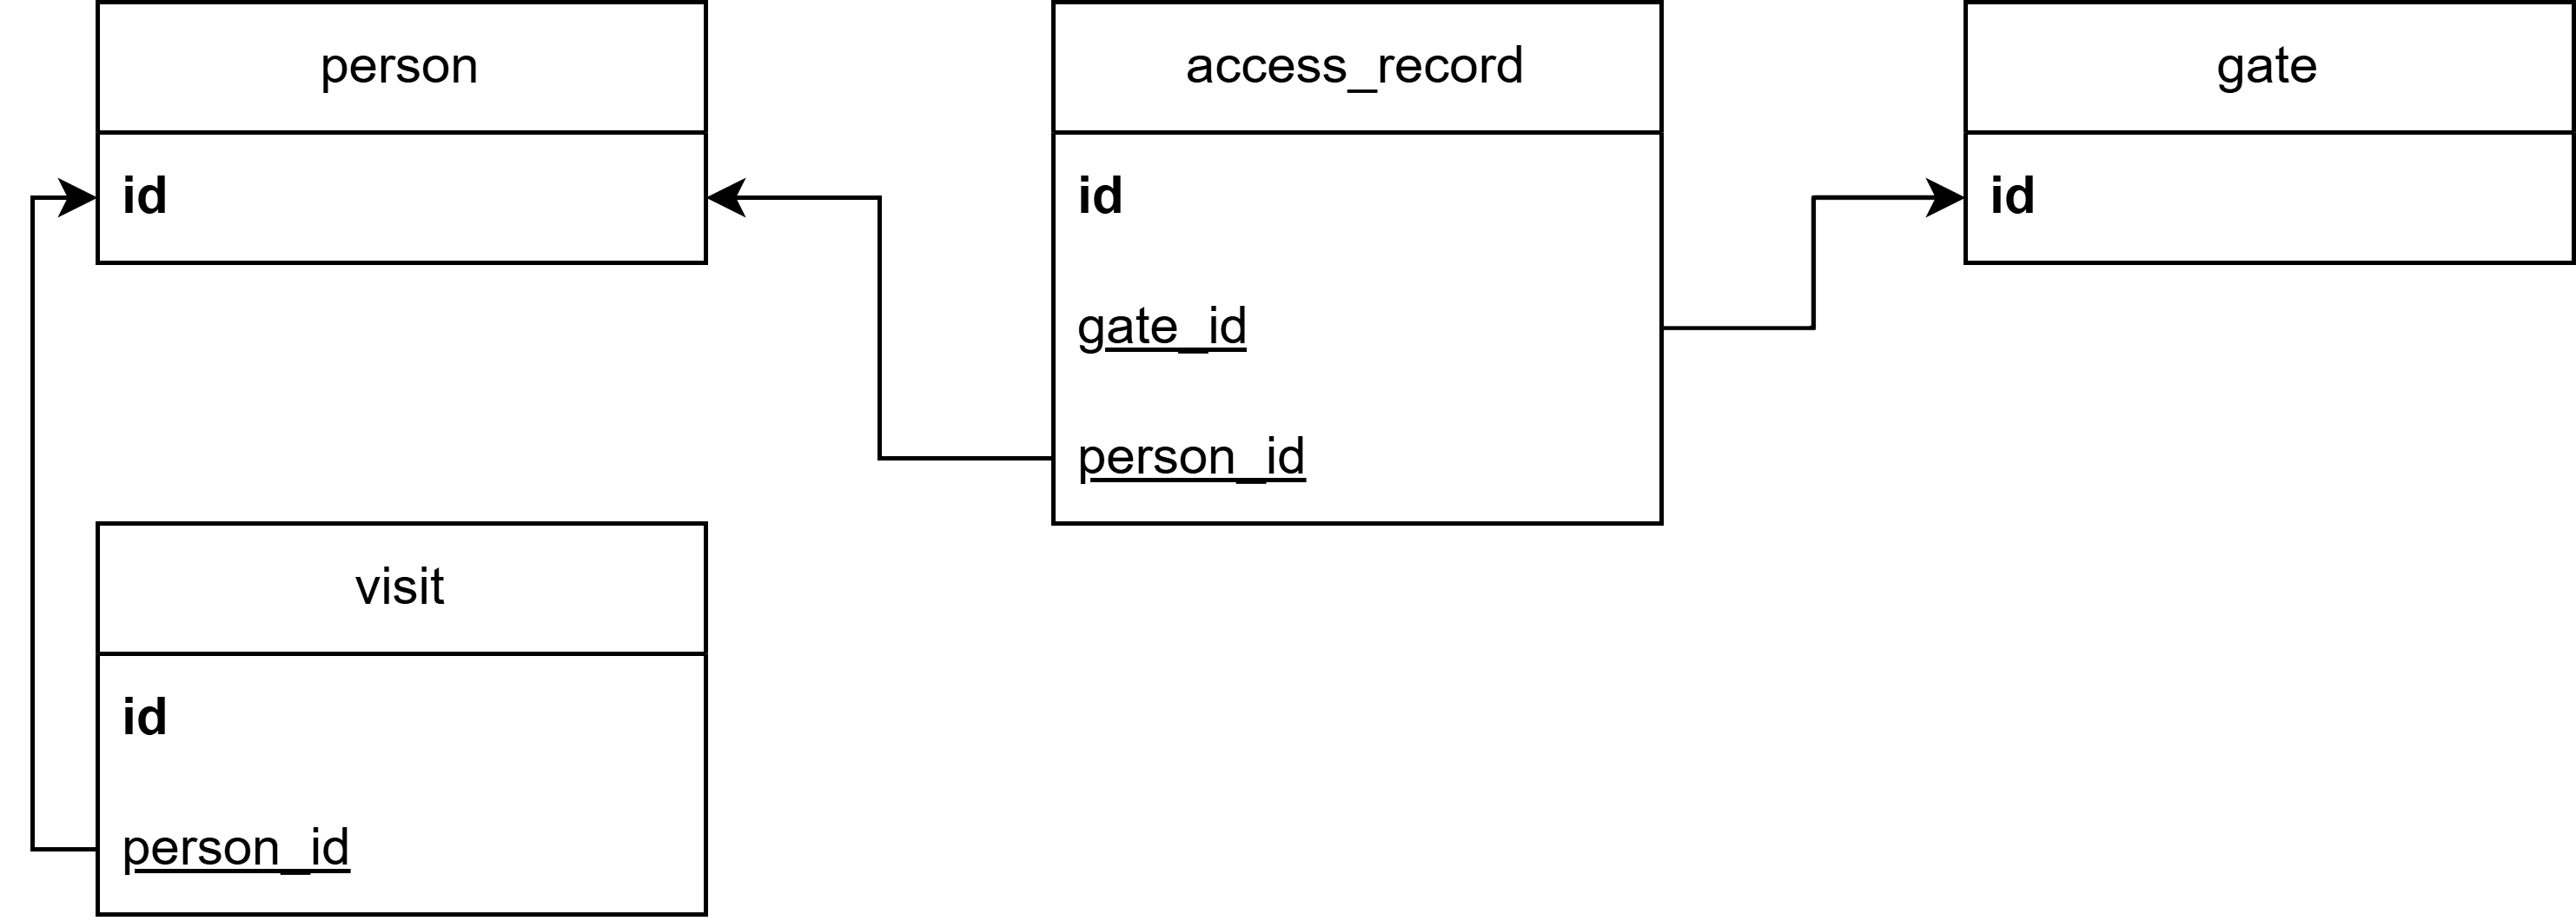
\includegraphics[width=0.9\textwidth]{images/erd_sistem.png}
    \vspace{4cm} % Placeholder untuk gambar ERD
    \caption{Entity Relationship Diagram (ERD) Sistem Manajemen Akses}
    \label{fig:erd_sistem}
\end{figure}

Sistem membedakan dua jenis data visual: (1) Foto Profil yang disimpan pada tabel \textit{person} sebagai referensi identitas saat pendaftaran, dan (2) Foto Snapshot yang disimpan pada tabel \textit{access\_record} sebagai bukti audit otomatis hanya pada saat terjadi kejadian anomali. Untuk menjamin performa pengambilan data pada skala log yang besar, sistem menerapkan teknik pengindeksan (\textit{indexing}) pada kolom \textit{time} dan \textit{person\_id}. Hal ini memungkinkan proses pencarian riwayat pergerakan dan pembuatan laporan agregat tetap berjalan responsif meskipun volume data transaksi terus meningkat.

\subsection{Kamus Data}
Detail spesifikasi teknis dari setiap tabel basis data didefinisikan melalui kamus data berikut:

\begin{table}[t]
    \centering
    \caption{Kamus Data Tabel \textit{person}}
    \label{tab:kamus_person}
    \begin{tabular}{|l|l|p{8cm}|}
        \hline
        \textbf{Nama Kolom} & \textbf{Tipe Data} & \textbf{Keterangan} \\
        \hline
        employeeNo & VarChar(32) & ID unik utama yang disinkronkan dengan terminal (Primary Key). \\
        \hline
        name & VarChar(128) & Nama lengkap karyawan atau tamu. \\
        \hline
        userType & Enum & Jenis pengguna (normal, visitor, atau blackList). \\
        \hline
        gender & Enum & Jenis kelamin pengguna (male, female, unknown). \\
        \hline
        validEnable & Boolean & Status keaktifan akun pada terminal gerbang. \\
        \hline
        validBeginTime & DateTime & Batas awal waktu validitas akses. \\
        \hline
        validEndTime & DateTime & Batas akhir waktu validitas akses. \\
        \hline
        photo\_path & VarChar(255) & Jalur penyimpanan file foto profil karyawan di server. \\
        \hline
    \end{tabular}
\end{table}
\begin{table}[t]
    \centering
    \caption{Kamus Data Tabel \textit{gate}}
    \label{tab:kamus_gate}
    \begin{tabular}{|l|l|p{8cm}|}
        \hline
        \textbf{Nama Kolom} & \textbf{Tipe Data} & \textbf{Keterangan} \\
        \hline
        id & UUID & Identifier unik internal untuk setiap gerbang (Primary Key). \\
        \hline
        device\_id & String & ID unik perangkat yang ditetapkan oleh sistem. \\
        \hline
        name & VarChar(128) & Nama deskriptif lokasi gerbang (misal: Lobi Jalur 1). \\
        \hline
        ip\_address & VarChar(64) & Alamat IP terminal gerbang di jaringan lokal. \\
        \hline
        username & VarChar(64) & Kredensial akun untuk otentikasi ISAPI. \\
        \hline
        password & VarChar(128) & Kata sandi perangkat (disimpan dalam bentuk terenkripsi). \\
        \hline
        direction & Enum & Arah akses gerbang (IN atau OUT). \\
        \hline
    \end{tabular}
\end{table}
\begin{table}[H]
    \centering
    \caption{Kamus Data Tabel \textit{access\_record}}
    \label{tab:kamus_access_record}
    \begin{tabular}{|l|l|p{8cm}|}
        \hline
        \textbf{Nama Kolom} & \textbf{Tipe Data} & \textbf{Keterangan} \\
        \hline
        serialNo & VarChar(128) & Nomor seri unik kejadian dari protokol ISAPI (Primary Key). \\
        \hline
        major & Int & Kode kategori kejadian (\textit{Major Event Code}). \\
        \hline
        minor & Int & Kode spesifik kejadian (\textit{Minor Event Code}). \\
        \hline
        time & DateTime & Stempel waktu saat akses terjadi di gerbang. \\
        \hline
        person\_id & VarChar(32) & Relasi ke identitas karyawan (Foreign Key ke \textit{person}). \\
        \hline
        gate\_id & UUID & Relasi ke terminal gerbang (Foreign Key ke \textit{gate}). \\
        \hline
        snapshot\_path & VarChar(255) & Jalur penyimpanan foto bukti anomali di server. \\
        \hline
        is\_processed & Boolean & Status pemrosesan data untuk kebutuhan analitik. \\
        \hline
    \end{tabular}
\end{table}
\begin{table}[t]
    \centering
    \caption{Kamus Data Tabel \textit{account}}
    \label{tab:kamus_account}
    \begin{tabular}{|l|l|p{8cm}|}
        \hline
        \textbf{Nama Kolom} & \textbf{Tipe Data} & \textbf{Keterangan} \\
        \hline
        id & UUID & Identifier unik internal akun administrator (Primary Key). \\
        \hline
        name & VarChar(128) & Nama lengkap administrator sistem. \\
        \hline
        username & VarChar(64) & Nama pengguna untuk masuk ke \textit{dashboard} (Unique). \\
        \hline
        password & VarChar(255) & Kata sandi akun (disimpan menggunakan algoritma \textit{hashing} bcrypt). \\
        \hline
        createdAt & DateTime & Stempel waktu pembuatan akun. \\
        \hline
    \end{tabular}
\end{table}
\begin{table}[H]
    \centering
    \caption{Kamus Data Tabel \textit{visit}}
    \label{tab:kamus_visit}
    \begin{tabular}{|l|l|p{8cm}|}
        \hline
        \textbf{Nama Kolom} & \textbf{Tipe Data} & \textbf{Keterangan} \\
        \hline
        id & UUID & Identifier unik rekaman kunjungan (Primary Key). \\
        \hline
        person\_id & VarChar(32) & Relasi ke subjek akses (Foreign Key ke \textit{person}). \\
        \hline
        entry\_time & DateTime & Stempel waktu pertama subjek memasuki gedung pada hari tersebut. \\
        \hline
        exit\_time & DateTime & Stempel waktu terakhir subjek keluar dari gedung. \\
        \hline
        status & Enum & Status kehadiran (ACTIVE, COMPLETED, dsb). \\
        \hline
    \end{tabular}
\end{table}

\subsection{Integritas Relasional dan Aturan Bisnis}
Untuk menjaga kualitas data, sistem menerapkan standarisasi nilai melalui penggunaan tipe data terstruktur (\textit{enum}) dan aturan integritas relasional sebagai berikut:

\begin{table}[H]
    \centering
    \caption{Definisi Tipe Data Terstruktur (\textit{Enum})}
    \label{tab:definisi_enum}
    \begin{tabular}{|l|l|p{7cm}|}
        \hline
        \textbf{Nama Enum} & \textbf{Nilai yang Diperbolehkan} & \textbf{Fungsi} \\
        \hline
        UserType & normal, visitor, blackList & Mengategorikan subjek akses. \\
        \hline
        Gender & male, female, unknown & Standarisasi jenis kelamin biometrik. \\
        \hline
        GateDirection & IN, OUT & Menentukan arah lalu lintas gerbang. \\
        \hline
        VisitStatus & ACTIVE, COMPLETED, EMERGENCY, EVACUATED & Melacak status kehadiran dan progres evakuasi personel. \\
        \hline
    \end{tabular}
\end{table}

\begin{enumerate}
    \item \textbf{Integritas Riwayat Akses:} Sistem menerapkan aturan \textit{Restricted Delete} pada relasi antara profil karyawan dan log pergerakan. Hal ini memastikan bahwa riwayat akses tidak akan hilang dari basis data meskipun data identitas karyawan dihapus dari memori terminal gerbang, guna menjaga akuntabilitas audit keamanan.
    \item \textbf{Strategi \textit{Safe Sweep}:} Sebagai bagian dari integritas data, penghapusan otomatis terhadap profil yang tidak lagi terdeteksi di perangkat keras melalui algoritma \textit{Mark \& Sweep} hanya akan dilakukan jika subjek tersebut tidak memiliki riwayat log akses dalam basis data. Hal ini menjamin bahwa seluruh data transaksi masa lalu tetap tersimpan secara utuh untuk kebutuhan investigasi keamanan siber.
    \item \textbf{Mekanisme Pembersihan Atomik (\textit{Atomic Cleanup}):} Sistem menjamin kebersihan data melalui prosedur penghapusan serentak. Ketika sebuah profil karyawan dihapus melalui antarmuka web, \textit{middleware} secara otomatis mencabut hak akses pada memori fisik terminal, menghapus rekaman terkait di basis data, serta memusnahkan file fisik foto profil dari media penyimpanan server guna mematuhi prinsip minimasi data.
\end{enumerate}

\section{Perancangan Logika Program}
Perancangan logika program mendefinisikan alur kerja otomatisasi pada lapisan aplikasi (\textit{middleware}) untuk menjalankan fungsi sinkronisasi data dan pemrosesan kejadian akses secara mandiri.

\subsection{Logika Sinkronisasi Identitas (\textit{Mark \& Sweep})}
Untuk menjaga konsistensi data antara basis data server dengan memori terminal gerbang, sistem menerapkan algoritma \textit{Mark \& Sweep}. Logika ini bekerja dalam dua fase utama. Pertama, fase \textit{mark} (penandaan) di mana sistem menarik seluruh daftar ID karyawan dari terminal dan memperbarui stempel waktu sinkronisasi (\textit{last synced at}) pada tabel \textit{person}. Kedua, fase \textit{sweep} (penyisiran) di mana sistem mencari rekaman yang stempel waktunya tidak diperbarui pada fase pertama, yang mengindikasikan bahwa data tersebut telah dihapus secara manual dari terminal gerbang. Sistem kemudian akan menghapus rekaman tersebut dari basis data server secara otomatis (dengan tetap memperhatikan integritas riwayat log). Alur algoritma ini diilustrasikan pada Gambar 4.4.

\begin{figure}[H]
    \centering
    % \includegraphics[width=0.7\textwidth]{images/flowchart_mark_sweep.png}
    \vspace{4cm} % Placeholder untuk flowchart Mark & Sweep
    \caption{Diagram Alir Algoritma \textit{Mark \& Sweep}}
    \label{fig:flowchart_mark_sweep}
\end{figure}

\subsection{Logika Pemrosesan Kejadian Akses dan Deteksi Anomali}
Sistem melakukan pemantauan lalu lintas secara aktif melalui mekanisme penjadwalan setiap 10 detik. Logika ini dirancang untuk menarik seluruh kejadian terbaru (\textit{AcsEvent}) dari protokol ISAPI. Setiap log yang ditarik akan melewati proses validasi untuk menghindari duplikasi data berdasarkan nomor seri kejadian (\textit{serialNo}). Jika sistem mendeteksi kejadian dengan kode \textit{minor} yang mengindikasikan kegagalan akses (misalnya wajah tidak terdaftar atau periode validitas habis), sistem secara otomatis memicu fungsi pengambilan data biner untuk mengunduh foto cuplikan (\textit{snapshot}) pelaku dari terminal. Hasil pemrosesan log ini kemudian dikirimkan ke \textit{dashboard} melalui jalur \textit{Socket.IO} secara \textit{real-time}. Diagram alir pemrosesan log dapat dilihat pada Gambar 4.5.

Untuk menjamin keandalan (\textit{reliability}) arsitektur ini pada lingkungan operasional fisik, logika penjadwalan juga dilengkapi dengan beberapa mekanisme tambahan:
\begin{enumerate}
    \item Penanganan Otentikasi Dinamis (\textit{Auth Retry Logic}): Komunikasi dengan terminal biometrik sering kali dihadapkan pada tantangan penolakan awal (\textit{401 Unauthorized}) yang merupakan sifat bawaan dari protokol \textit{Digest Authentication}. \textit{Middleware} dirancang untuk menangkap penolakan tersebut secara terprogram, menghitung ulang respon kriptografi yang diminta, dan melakukan pengiriman ulang (\textit{retry}) secara otomatis tanpa menggagalkan proses penarikan data secara keseluruhan.
    \item Toleransi Kesalahan (\textit{Fault Tolerance}): Seluruh siklus komunikasi dibungkus dalam mekanisme penanganan eksepsi (\textit{try-catch block}). Hal ini memastikan bahwa apabila terjadi gangguan jaringan lokal atau terminal fisik kehilangan daya listrik, layanan \textit{backend} NestJS tidak akan mengalami \textit{crash}, melainkan hanya akan mencatat peringatan pada log internal dan melanjutkan rutinitas pemantauan pada interval 10 detik berikutnya. Mekanisme ini juga mendukung ketahanan parsial (\textit{partial resilience}), di mana kegagalan komunikasi pada salah satu terminal tidak akan menghentikan siklus pemantauan pada terminal lainnya.
    \item Penanganan Aliran Data Biner (\textit{Binary Stream Handling}): Saat pemicu anomali aktif, sistem menjalankan fungsi pemrosesan data biner untuk mengunduh bukti visual. Proses ini mencakup penangkapan aliran data (\textit{stream}) dari gerbang, penulisan file fisik pada direktori penyimpanan server, serta sinkronisasi jalur lokasi file tersebut ke dalam basis data secara atomik.
    \item Diseminasi Data \textit{Real-time} (\textit{Data Broadcast}): Pasca pemrosesan log berhasil disimpan ke dalam basis data, sistem melakukan penyebaran informasi secara instan melalui gerbang \textit{Socket.IO}. Hal ini menjamin bahwa setiap kejadian akses terbaru akan muncul secara otomatis pada layar pemantauan tanpa intervensi manual dari pengguna.
    \item Otentikasi Dinamis Proaktif (\textit{Fresh-Challenge}): Mengingat karakteristik protokol \textit{Digest Authentication} yang berbasis sesi dinamis, \textit{middleware} dirancang untuk selalu melakukan negosiasi kredensial baru pada setiap siklus permintaan. Sistem mampu merespon tantangan otentikasi (\textit{401 Challenge}) dari terminal secara instan dengan menghasilkan \textit{hash} kriptografi yang segar, sehingga menjamin akses data tetap berjalan lancar meskipun terjadi pergantian sesi pada perangkat keras.
    \item Logika Pemetaan Protokol (\textit{Event Mapping}): Mengingat terminal mengirimkan rekaman kejadian dalam bentuk kode numerik mentah (\textit{Major/Minor Code}), sistem melakukan pemetaan (\textit{mapping}) secara dinamis. Logika ini mengubah kode-kode biner tersebut menjadi terminologi yang dipahami pengguna (seperti 'Wajah Cocok', 'Kartu Tidak Terdaftar', atau 'Otentikasi Gagal') sebelum data disajikan pada antarmuka \textit{dashboard}.
    \item Logika Sinkronisasi Adaptif (\textit{Upsert Fallback}): Selama proses pendaftaran identitas, sistem menerapkan logika adaptif. Apabila perintah pembuatan rekaman baru (\textit{POST}) ditolak oleh terminal karena data subjek telah ada di memori perangkat, sistem secara otomatis melakukan pengalihan ke perintah pembaruan (\textit{PUT}) guna menjamin keberhasilan sinkronisasi tanpa kegagalan proses.
    \item Logika Integritas Rekaman Yatim (\textit{Orphan Record Handling}): Untuk menjamin tidak adanya kehilangan data transaksi, sistem secara otomatis akan membuat profil identitas sementara (\textit{Unknown Stub}) apabila terdeteksi adanya rekaman log dari subjek yang belum terdaftar di basis data lokal. Hal ini memastikan setiap aktivitas pergerakan tetap terdokumentasi dan dapat diaudit di kemudian hari.
    \item Logika Translasi Format Data (\textit{Payload Serialization}): Mengingat terminal perangkat keras beroperasi menggunakan protokol berbasis XML untuk perintah tertentu, sementara arsitektur web modern menggunakan JSON, \textit{middleware} mengimplementasikan fungsi translasi otomatis. Logika ini menerjemahkan objek JSON dari basis data maupun \textit{frontend} menjadi struktur \textit{Extensible Markup Language} (XML) yang dapat diproses oleh terminal guna menjamin interoperabilitas sistem.
    \item Logika Isolasi Modul (\textit{Module Isolation}): Untuk menjaga ketajaman ruang lingkup penelitian, \textit{middleware} menerapkan filter ketat terhadap tipe pengguna. Sistem dirancang untuk secara otomatis menyaring data dari basis data bersama sehingga hanya rekaman aktivitas milik subjek karyawan (\textit{normal user}) yang diproses dan disajikan pada antarmuka pemantauan, menjamin privasi dan relevansi informasi bagi pengelola SDM.
    \item Logika Pencegahan Balapan Proses (\textit{Race Condition Prevention}): Mengingat interval sinkronisasi yang sangat singkat (10 detik), sistem menerapkan mekanisme kunci (\textit{locking mechanism}). \textit{Middleware} akan memantau status eksekusi aktif dan secara otomatis membatalkan siklus penjadwalan baru apabila siklus sebelumnya belum selesai diproses, guna mencegah terjadinya penumpukan beban memori pada server.
    \item Logika Pemrosesan Berkelompok (\textit{Batch Processing}): Untuk menjaga stabilitas kinerja saat menangani volume data yang besar, sistem melakukan pemrosesan log secara bertahap. Logika ini membatasi jumlah antrean data dalam satu siklus eksekusi (misalnya maksimal 1.000 rekaman), sehingga konsumsi sumber daya komputasi tetap terkendali dan respon sistem tetap optimal.
    \item Logika Konstruksi Protokol Manual (\textit{Custom Multipart Handling}): Untuk mengatasi ketatnya pembacaan data biner pada \textit{firmware} terminal, sistem tidak menggunakan pustaka pengiriman file standar. \textit{Middleware} merangkai struktur \textit{boundary} dan \textit{metadata header} secara manual pada level biner guna menjamin kompatibilitas permintaan pengunggahan data wajah yang spesifik terhadap parser protokol perangkat keras.
\end{enumerate}

\begin{figure}[H]
    \centering
    % \includegraphics[width=0.7\textwidth]{images/flowchart_event_polling.png}
    \vspace{4cm} % Placeholder untuk flowchart Event Polling
    \caption{Diagram Alir Pemrosesan Kejadian Akses dan Deteksi Anomali}
    \label{fig:flowchart_event_polling}
\end{figure}

\subsection{Logika Agregasi Kunjungan (\textit{Visit Aggregation})}
Sistem mengimplementasikan proses \textit{Extract, Transform, Load} (ETL) untuk mengubah data mentah dari \textit{access\_record} menjadi informasi kehadiran harian yang terstruktur pada tabel \textit{visit}. Logika ini mendeteksi pasangan aktivitas masuk dan keluar untuk setiap individu guna mempermudah pembuatan laporan riwayat kehadiran secara sistematis. Rekaman status \textit{ACTIVE} akan dibuat saat kejadian masuk (\textit{entry}) terdeteksi, dan akan diperbarui stempel waktu selesainya serta diubah statusnya menjadi \textit{COMPLETED} saat kejadian keluar (\textit{exit}) yang bersangkutan terekam oleh sistem pada hari yang sama. Proses transformasi ini dijalankan menggunakan mekanisme transaksi basis data (\textit{Database Transaction}). Hal ini menjamin sifat atomik pada setiap siklus pemrosesan, di mana pembaruan status log mentah dan pembuatan rekaman kunjungan dilakukan secara serentak guna mencegah terjadinya inkonsistensi data apabila terjadi kegagalan sistem di tengah proses eksekusi.

\subsection{Logika Agregasi Visual Dashboard}
Untuk meningkatkan keterbacaan data bagi administrator, sistem menerapkan logika agregasi visual pada antarmuka pemantauan. Beberapa kejadian akses (masuk dan keluar) dari subjek yang sama pada hari operasional yang sama dikonsolidasikan menjadi satu baris informasi profil tunggal. Baris tersebut dilengkapi dengan linimasa pergerakan kronologis (\textit{timeline chips}), sehingga memudahkan pengelola dalam meninjau rincian aktivitas harian personel tanpa menyebabkan penumpukan baris data (\textit{data clutter}) pada layar.

\subsection{Kebijakan Retensi Rekaman Visual}
Untuk menjaga efisiensi ruang penyimpanan server and kepatuhan terhadap prinsip privasi data, sistem menerapkan kebijakan retensi otomatis (\textit{Automatic Pruning}). Logika ini secara periodik memindai direktori penyimpanan \textit{snapshot} anomali dan memusnahkan file gambar yang telah melampaui masa simpan tertentu (misalnya 30 hari). Proses pembersihan ini hanya menyasar pada aset fisik biner tanpa menghapus rekaman metadata tekstual pada basis data, sehingga akuntabilitas audit riwayat tetap terjaga tanpa membebani kapasitas penyimpanan jangka panjang.

\subsection{Logika Pencegahan Duplikasi Akses (\textit{Access Debounce})}
Guna menjaga kebersihan data riwayat pergerakan harian, sistem menerapkan mekanisme waktu jeda (\textit{cooldown}) selama 60 detik. Apabila terdeteksi adanya aktivitas pemindaian biometrik berulang dari subjek yang sama di terminal yang sama dalam rentang waktu tersebut, sistem secara otomatis akan mengabaikan kejadian tersebut. Logika ini krusial untuk mencegah timbulnya data duplikat (\textit{spam logs}) akibat perilaku pengguna yang melakukan pemindaian berulang sebelum gerbang tertutup sepenuhnya.

\subsection{Logika Agregasi Laporan Karyawan}
Sistem menyediakan fungsi pemrosesan data khusus untuk kebutuhan pelaporan administratif. Logika ini secara cerdas menyaring seluruh rekaman log mentah untuk menentukan stempel waktu masuk pertama (\textit{first-in}) dan keluar terakhir (\textit{last-out}) setiap karyawan pada hari operasional tertentu. Hasil pemrosesan ini kemudian dikonversi menjadi dokumen digital (CSV) yang menyajikan ringkasan trafik harian serta linimasa pergerakan personel secara kronologis guna mempermudah evaluasi riwayat kehadiran oleh pihak manajemen.

\section{Perancangan Antarmuka Pengguna}
Perancangan antarmuka pengguna (\textit{UI/UX}) diarahkan untuk memberikan kemudahan bagi administrator dalam melakukan pemantauan dan pengelolaan data karyawan secara intuitif. Antarmuka ini dibangun menggunakan komponen yang responsif guna menjamin kenyamanan akses melalui berbagai perangkat peramban web (\textit{Responsive Web Design}), serta mengadopsi mekanisme interaksi berbasis dialog (\textit{Modal-based interaction}) guna menjaga fokus pengelola terhadap data pemantauan utama dan menyederhanakan alur kerja administratif.

\subsection{Antarmuka Pemantauan Akses Karyawan}
Halaman ini merupakan pusat kendali operasional yang menyajikan data pergerakan log secara \textit{real-time}. Rancangan halaman ini terdiri dari beberapa komponen utama:
\begin{enumerate}
    \item Widget Jam Digital (\textit{Live Clock WIB}): Komponen penunjuk waktu \textit{real-time} yang berfungsi sebagai acuan tunggal zona waktu Asia/Jakarta untuk seluruh aktivitas sinkronisasi data.
    \item Ringkasan Statistik: Menyajikan kartu informasi yang menunjukkan jumlah subjek yang berada di dalam gedung dan jumlah kejadian anomali pada hari berjalan.
    \item Grafik Tren Aktivitas: Visualisasi dalam bentuk diagram batang yang menyajikan tren lalu lintas pergerakan (\textit{in/out}) dan kejadian anomali setiap jam. Komponen ini dilengkapi dengan fitur penanda jam aktif (\textit{Active Hour Highlight}) yang memberikan aksen visual berbeda pada waktu berjalan guna mempermudah pemantauan fluktuasi trafik harian.
    \item Daftar Agregasi Pergerakan: Komponen visual yang menyajikan data secara terkelompok berdasarkan subjek (\textit{person-centric}). Setiap profil dilengkapi dengan deretan penanda (\textit{timeline chips}) yang meringkas urutan waktu kejadian masuk dan keluar individu tersebut dalam satu hari operasional.
    \item Tabel Arsip Kronologis: Tabel dinamis yang menyajikan seluruh rekaman log secara berurutan berdasarkan waktu kejadian (\textit{event-centric}). Komponen ini berfungsi untuk kebutuhan audit mendalam dan terintegrasi langsung dengan fitur pencarian serta paginasi.
    \item Kendali Pelaporan (\textit{Export Tools}): Komponen tombol aksi yang memungkinkan administrator untuk melakukan ekstraksi data riwayat pergerakan ke dalam format dokumen digital secara instan berdasarkan filter rentang waktu yang dipilih.
    \item Fitur Pencarian dan Penapisan (\textit{Filtering}): Antarmuka navigasi yang memungkinkan pengelola untuk melakukan pencarian subjek secara spesifik serta membatasi tampilan log berdasarkan parameter tanggal tertentu guna mempercepat proses audit.
    \item Komponen Paginasi (\textit{Pagination}): Mekanisme navigasi tabel yang membagi penyajian data log ke dalam beberapa halaman terkendali guna menjaga performa pemuatan antarmuka saat menangani volume data yang besar.
    \item Standarisasi Kode Warna: Penerapan skema warna visual (\textit{visual semantic}) untuk mempercepat identifikasi arah pergerakan, di mana warna hijau (\textit{emerald}) digunakan untuk penanda masuk dan warna biru digunakan untuk penanda keluar.
    \item Penanganan Data Kosong (\textit{Empty State}): Antarmuka dirancang untuk tetap informatif meskipun belum terdapat aktivitas terekam, dengan menyajikan komponen penahan tempat (\textit{placeholder}) yang menjelaskan ketiadaan data riwayat kepada pengguna.
    \item Status Terminal: Indikator visual yang memantau kesehatan koneksi setiap perangkat gerbang di lobi guna mempermudah deteksi gangguan teknis secara dini.
    \item Navigasi Kalender Riwayat: Komponen pemilihan tanggal yang memungkinkan pengelola untuk meninjau data pergerakan dan statistik dari hari-hari operasional sebelumnya, memberikan fleksibilitas dalam proses audit kejadian masa lalu.
\end{enumerate}

Rancangan tata letak antarmuka pemantauan diilustrasikan pada Gambar 4.6.

\begin{figure}[H]
    \centering
    % 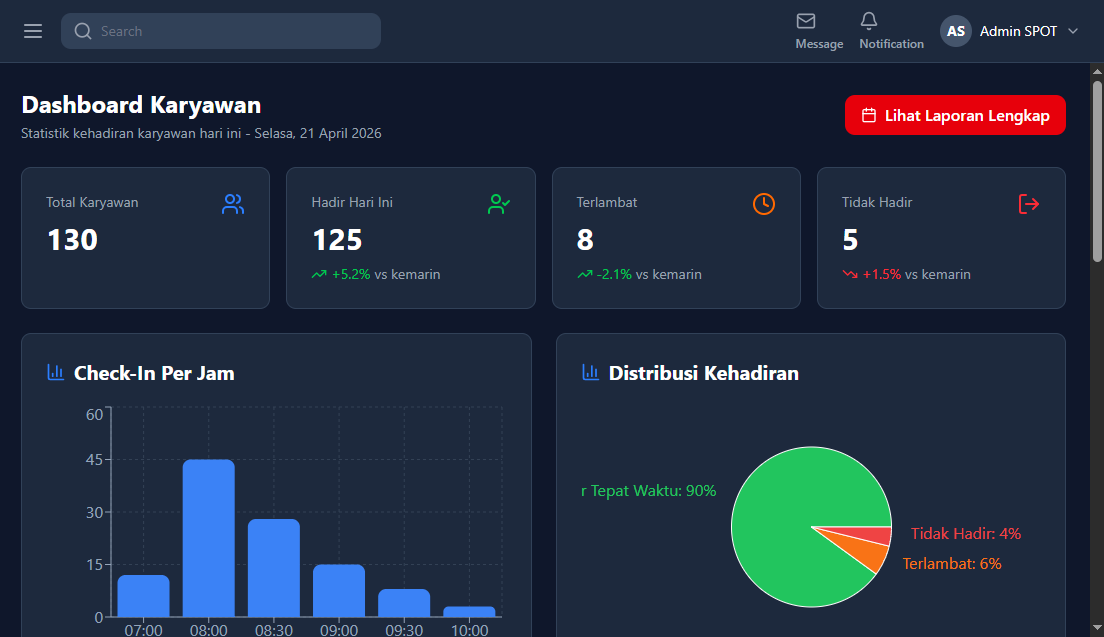
\includegraphics[width=0.9\textwidth]{images/mockup_dashboard.png}
    \vspace{4cm} % Placeholder untuk mockup dashboard
    \caption{Rancangan Antarmuka Dashboard Pemantauan}
    \label{fig:mockup_dashboard}
\end{figure}

\subsection{Antarmuka Manajemen Identitas Karyawan}
Halaman ini dirancang untuk memfasilitasi administrasi data biometrik secara terpusat. Fitur utama pada antarmuka ini meliputi:
\begin{enumerate}
    \item Formulir Pendaftaran: Antarmuka input untuk merekam data identitas baru yang mencakup nomor karyawan, nama lengkap, jenis kelamin, serta pengunggahan file foto wajah.
    \item Fitur Pencarian Profil: Komponen masukan teks pada daftar master karyawan yang memungkinkan administrator untuk mengisolasi subjek tertentu berdasarkan nama atau nomor identitas secara \textit{real-time}.
    \item Kendali Aksi Dinamis: Deretan tombol aksi pada setiap baris data yang memungkinkan pengelola untuk melakukan pembaruan informasi (\textit{edit}) atau penghapusan profil secara instan.
    \item Dialog Konfirmasi Penghapusan: Mekanisme pengamanan operasional berupa jendela peringatan berwarna kontras (merah) yang mewajibkan admin mengonfirmasi tindakan sebelum sistem memusnahkan data dari basis data dan memori fisik terminal secara permanen.
    \item Indikator Sinkronisasi Multiterminal: Komponen umpan balik visual yang menunjukkan status distribusi data identitas subjek pada setiap gerbang biometrik yang terhubung dalam jaringan, guna memastikan konsistensi data di seluruh titik akses.
    \item Galeri Identitas: Daftar profil yang menyajikan pratinjau foto profil master guna mempermudah verifikasi administratif oleh pengelola gedung.
    \item Umpan Balik Proses (\textit{Action Feedback}): Mekanisme pencegahan kesalahan yang menonaktifkan kontrol antarmuka (\textit{disabled state}) dan menampilkan indikator pemuatan (\textit{loading state}) selama proses sinkronisasi ke perangkat keras berlangsung.
    \item Umpan Balik Status (\textit{Status Toasts}): Penggunaan notifikasi ringkas (\textit{toasts}) untuk mengonfirmasi keberhasilan pendaftaran atau menjelaskan alasan kegagalan koneksi perangkat keras secara instan guna menjamin transparansi status operasi.
\end{enumerate}

Rancangan halaman manajemen identitas diilustrasikan pada Gambar 4.7.

\begin{figure}[H]
    \centering
    % \includegraphics[width=0.9\textwidth]{images/mockup_management.png}
    \vspace{4cm} % Placeholder untuk mockup management
    \caption{Rancangan Antarmuka Manajemen Profil Karyawan}
    \label{fig:mockup_management}
\end{figure}

\subsection{Visualisasi Audit Anomali}
Untuk mendukung fungsi investigasi keamanan, sistem menyertakan komponen visualisasi khusus untuk mendokumentasikan pelanggaran akses. Fitur ini diimplementasikan melalui dialog verifikasi keamanan (\textit{Security Verification Dialog}) yang muncul secara interaktif. Saat sensor gerbang mendeteksi anomali, sistem akan menyajikan foto cuplikan (\textit{snapshot}) wajah pelaku yang ditangkap secara otomatis oleh kamera gerbang dalam bingkai visual dengan aksen warna kontras (merah). Visualisasi ini menyertakan metadata rincian pelanggaran (waktu, lokasi gerbang, dan alasan penolakan), sehingga memungkinkan petugas keamanan melakukan verifikasi visual secara cepat guna mengidentifikasi pihak yang mencoba masuk tanpa izin yang sah.

\section{Perancangan Antarmuka Komunikasi (API)}
Perancangan antarmuka komunikasi mendefinisikan standar pertukaran data antar komponen dalam sistem manajemen akses. Jalur komunikasi dibagi menjadi tiga kategori utama untuk menjamin integritas fungsionalitas \textit{middleware}.

\subsection{Arsitektur RESTful API}
Komunikasi antara antarmuka pengguna (\textit{frontend}) dengan layanan pusat (\textit{backend}) dilakukan melalui protokol HTTP berbasis \textit{RESTful API}. Sistem mendukung dua format komunikasi utama: format JSON untuk pertukaran data tekstual reguler, serta format \textit{multipart/form-data} yang dikhususkan untuk transmisi data biometrik visual saat pendaftaran profil. Selain pengiriman data utama, respon API juga dilengkapi dengan metadata navigasi (seperti jumlah total rekaman dan informasi paginasi) untuk menjamin efisiensi komunikasi data saat \textit{frontend} menangani ribuan baris log riwayat pergerakan. Seluruh permintaan data tersebut dilindungi oleh lapisan otentikasi JWT pada setiap titik akhirnya. Sebagai catatan khusus, pada rute ekstraksi laporan (ekspor), token otentikasi dikirimkan melalui parameter kueri (\textit{query parameter}) untuk mengakomodasi batasan teknis pada mekanisme pengunduhan file melalui jendela peramban baru. Selain itu, sistem menerapkan kebijakan \textit{Cross-Origin Resource Sharing} (CORS) untuk membatasi interaksi API hanya pada domain resmi yang terdaftar guna mencegah eksploitasi akses dari sumber luar yang tidak sah. Untuk menjamin respon antarmuka yang instan, rute pemantauan status gerbang mengadopsi mekanisme penyimpanan sementara (\textit{Caching}). Server menyajikan data status kesehatan perangkat dari memori \textit{cache} yang diperbarui secara asinkron, sehingga meminimalkan beban komputasi langsung pada unit terminal saat terjadi permintaan akses data dari banyak klien secara serentak. Setiap respon API juga mengadopsi standar kode status HTTP (\textit{HTTP Status Codes}) guna memfasilitasi penanganan kesalahan dan umpan balik pengguna yang akurat pada sisi klien. Terakhir, sistem menerapkan mekanisme verifikasi kriptografi pada lapisan terluar antarmuka pengguna (\textit{Edge Security}). Menggunakan pustaka \textit{jose} pada \textit{middleware} Next.js, setiap permintaan data divalidasi keaslian tanda tangan tokennya secara mandiri sebelum diteruskan ke server pusat, guna mencegah upaya pemalsuan identitas administrator melalui manipulasi \textit{cookie} peramban. Khusus pada rute ekstraksi data, sistem melakukan pemetaan ulang (\textit{Mapping}) dari kolom basis data teknis menjadi label informasi administratif guna menghasilkan dokumen laporan CSV yang siap guna bagi pihak manajemen. Sistem juga mengadopsi pola agregasi respon (\textit{Response Aggregation}) pada operasi multiterminal, di mana \textit{backend} akan mengonsolidasikan hasil eksekusi dari seluruh gerbang fisik ke dalam satu objek informasi tunggal sebelum dikirimkan ke \textit{frontend} guna mempermudah penyajian status sinkronisasi harian pada antarmuka administrator. Rancangan rute API utama dirangkum dalam Tabel \ref{tab:api_restful}.

\begin{table}[H]
    \centering
    \caption{Rancangan Titik Akhir (\textit{Endpoint}) RESTful API}
    \label{tab:api_restful}
    \begin{tabular}{|l|c|l|p{6cm}|}
        \hline
        \textbf{Endpoint} & \textbf{Metode} & \textbf{Akses} & \textbf{Fungsi} \\
        \hline
        /auth/login & POST & Publik & Otentikasi administrator dan pemberian token JWT. \\
        \hline
        /auth/profile & GET & Private & Mengambil metadata profil administrator yang sedang masuk. \\
        \hline
        /employees & GET & Private & Mengambil daftar seluruh profil karyawan dari basis data. \\
        \hline
        /employees/register & POST & Private & Mendaftarkan subjek baru beserta pengunggahan foto profil. \\
        \hline
        /employees/:id & PATCH & Private & Memperbarui informasi profil karyawan tertentu. \\
        \hline
        /employees/:id & DELETE & Private & Menghapus data karyawan secara atomik (DB dan Hardware). \\
        \hline
        /statistics/karyawan & GET & Private & Mengambil data statistik kehadiran dan grafik tren harian. \\
        \hline
        /statistics/karyawan/logs & GET & Private & Mengambil data riwayat pergerakan secara terpaginasi. \\
        \hline
        /statistics/karyawan/export & GET & Private & Melakukan ekstraksi data kehadiran ke dalam format CSV. \\
        \hline
        /gate-monitor/status & GET & Private & Memantau status kesehatan koneksi seluruh terminal gerbang. \\
        \hline
        /gate-control/:id/command & POST & Private & Mengirimkan instruksi kendali manual (buka/tutup) ke pintu gerbang. \\
        \hline
        /uploads/:folder/:file & GET & Private & Mengambil aliran data biner foto profil atau bukti visual anomali. \\
        \hline
    \end{tabular}
\end{table}

\subsection{Kanal Notifikasi \textit{Real-time}}
Untuk mendukung visualisasi tanpa pemuatan ulang (\textit{refresh}), sistem menyediakan jalur komunikasi dua arah menggunakan protokol \textit{WebSocket} melalui pustaka \textit{Socket.IO}. Kanal ini digunakan untuk mendorong pembaruan data secara proaktif dari server ke \textit{dashboard} segera setelah kejadian akses baru terdeteksi. Sesuai dengan standar keamanan siber, kanal ini dilindungi menggunakan mekanisme jabat tangan (\textit{handshake}) terotentikasi, di mana setiap klien wajib menyertakan token JWT yang valid guna mencegah penyadapan aliran data oleh pihak luar. Selain itu, distribusi data melalui kanal ini menggunakan mekanisme pembaruan atomik (\textit{Atomic Push}), di mana server hanya menyebarkan rekaman kejadian tunggal yang baru saja terproses guna mereduksi beban trafik jaringan dan menjamin respon visual yang instan. Detail kanal komunikasi ini disajikan pada Tabel \ref{tab:api_websocket}.

\begin{table}[t]
    \centering
    \caption{Rancangan Kanal Komunikasi \textit{Real-time} (Socket.IO)}
    \label{tab:api_websocket}
    \begin{tabular}{|l|c|p{8cm}|}
        \hline
        \textbf{Nama Event} & \textbf{Arah} & \textit{Keterangan} \\
        \hline
        events\_updated & Server $\rightarrow$ Client & Notifikasi pemicu penyegaran otomatis pada tabel log dan statistik dashboard. \\
        \hline
        gate\_status\_updated & Server $\rightarrow$ Client & Pengiriman status konektivitas (\textit{online/offline}) terbaru dari setiap gerbang. \\
        \hline
    \end{tabular}
\end{table}

\subsection{Integrasi Protokol ISAPI}
Interaksi antara server \textit{middleware} dengan perangkat keras terminal gerbang dilakukan melalui pemanggilan titik akhir (\textit{endpoint}) protokol ISAPI secara \textit{outbound}. Jalur ini digunakan untuk mengeksekusi perintah manajemen identitas dan penarikan log mentah. Seluruh integrasi dilakukan dengan menyertakan parameter kueri \textit{format=json} guna memastikan terminal memberikan respon dalam format yang terstandardisasi. Selain itu, permintaan data log dilakukan dengan menyertakan filter rentang waktu (\textit{Time-window Filtering}) yang spesifik, guna memastikan server hanya menarik rekaman terbaru dan menjaga efisiensi penggunaan lebar pita (\textit{bandwidth}) jaringan. Untuk menjamin efisiensi waktu pemrosesan harian, integrasi ISAPI juga dirancang menggunakan mekanisme orkestrasi paralel (\textit{Parallel Request Orchestration}). \textit{Middleware} melakukan pemanggilan titik akhir ke seluruh terminal gerbang secara serentak, sehingga total waktu eksekusi sinkronisasi tidak terakumulasi berdasarkan jumlah perangkat, melainkan hanya bergantung pada waktu respon terminal yang paling lambat. Mekanisme ini krusial untuk memastikan seluruh data dari keenam gerbang berhasil ditarik dalam jendela waktu penjadwalan 10 detik. Sistem juga menerapkan protokol pembungkusan data (\textit{JSON Wrapping}) yang berjenjang, di mana setiap informasi yang dikirimkan ke terminal disusun ke dalam objek \textit{root} spesifik guna memenuhi kriteria parser pada lapisan perangkat keras. Selain itu, sistem menerapkan aturan penyelarasan dialek protokol (\textit{Dialect Alignment}), di mana struktur data wajib mengikuti aturan penulisan kunci (\textit{Key Case-Sensitivity}) yang spesifik terhadap standar vendor (seperti penggunaan \textit{PascalCase} pada objek utama) guna memastikan instruksi dapat diuraikan secara tepat. Struktur integrasi ISAPI dirancang berdasarkan spesifikasi teknis vendor Hikvision sebagaimana tercantum dalam Tabel \ref{tab:api_isapi}. Selain itu, sistem menyertakan konfigurasi agen komunikasi yang fleksibel terhadap sertifikat keamanan perangkat keras pada jaringan lokal, memungkinkan pertukaran data terenkripsi (HTTPS) tetap berlangsung meskipun terminal menggunakan sertifikat \textit{self-signed} bawaan vendor.

\begin{table}[htbp]
    \centering
    \caption{Rancangan Integrasi Protokol ISAPI (\textit{Outbound})}
    \label{tab:api_isapi}
    \small
    \begin{tabularx}{\textwidth}{|>{\raggedright\arraybackslash}p{6cm}|c|X|}
        \hline
        \textbf{ISAPI Path} & \textbf{Metode} & \textbf{Tujuan Operasi} \\
        \hline
        \texttt{/ISAPI/\allowbreak AccessControl/\allowbreak AcsEvent} & POST & Melakukan pemindaian (polling) terhadap log kejadian terbaru. \\
        \hline
        \texttt{/ISAPI/\allowbreak AccessControl/\allowbreak AcsWorkStatus} & GET & Memantau status kesehatan terminal dan kondisi kunci pintu secara real-time. \\
        \hline
        \texttt{/ISAPI/\allowbreak AccessControl/\allowbreak UserInfo/\allowbreak Record} & POST/PUT & Menambahkan atau memperbarui identitas subjek pada memori terminal. \\
        \hline
        \texttt{/ISAPI/\allowbreak AccessControl/\allowbreak UserInfo/\allowbreak Search} & POST & Menarik daftar ID karyawan yang terdaftar untuk fase Mark. \\
        \hline
        \texttt{/ISAPI/\allowbreak AccessControl/\allowbreak UserInfo/\allowbreak Delete} & PUT & Mencabut hak akses subjek dari perangkat keras. \\
        \hline
        \texttt{/ISAPI/\allowbreak AccessControl/\allowbreak RemoteControl/\allowbreak door/1} & PUT & Melakukan instruksi pembukaan pintu secara jarak jauh (remote open). \\
        \hline
        \texttt{/ISAPI/\allowbreak Intelligent/\allowbreak FDLib/\allowbreak FaceDataRecord} & POST/PUT & Melakukan transmisi data biner (multipart) untuk pembaruan profil wajah pada terminal. \\
        \hline
        \texttt{/ISAPI/\allowbreak .../\allowbreak picture/\allowbreak ...} & GET & Mengunduh aset biner foto kejadian anomali berdasarkan referensi URL dinamis. \\
        \hline
    \end{tabularx}
\end{table}
